\newpage
\subsection{Simple Coloring}
\label{Coloring}
Beim \textit{Simple Coloring} wird für die betrachtete Ziffer nach Figuren gesucht, in denen diese Ziffer nur noch in zwei Kandidatenlisten vorkommt. Den Zellen dieser Kandidatenlisten werden dann zwei unterschiedliche Farben zugeordnet. Dadurch, dass sich die Kandidaten in den Figuren gegenseitig ausschließen, steht die betrachtete Ziffer immer in jedem Feld der entweder einen oder anderen Farbe.\\ 
Erster Widerspruch (Color Trap): In Zellen, die nicht gefärbt sind, die von beiden Farben gesehen werden und die die betrachtete Ziffer enthalten, kann diese gelöscht werden.\\
Zweiter Widerspruch (Color Wrap): Wenn eine Farbe in der gleichen Figur zwei mal vorkommt, dann können alle Vorkommen der Ziffer in Zellen mit dieser Farbe gelöscht werden, da die Ziffer entweder in allen Zellen steht oder in keiner. In allen Zellen kann die Ziffer nicht stehen, da eine Ziffer nicht zwei mal in einer Figur vorkommen kann.

\begin{figure}[h]
\begin{center}
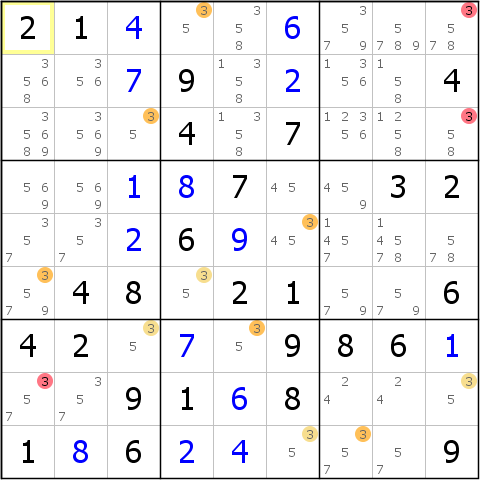
\includegraphics{./img/simple_coloring.png}
\caption{Simple Coloring - Color Trap}
\end{center}
\end{figure}

\noindent In \textbf{Abbildung 3.17}\footnote{Beispiel aus \cite{HDKColoring}} wird die Ziffer 3 betrachtet. Sie kann entweder in allen dunkelgelb oder allen hellgelb gefärbten Zellen stehen. Wir betrachten nun zwei Fälle. Wenn die Ziffer 3 in z8s9 steht, dann sind die Kandidaten in z8s1, z1s9 und z3s9 ausgeschlossen. Wenn nicht, dann muss sie in allen dunkelgelb gefärbten Zellen stehen, insbesondere in z1s4 und z3s3. Diese schließen ebenfalls die rot markierten Kandidaten aus. Damit können diese in keinem Fall in z1s9 und z3s9 stehen und können gelöscht werden.